\documentclass[aspectratio=169,11pt]{beamer}
\usetheme[progressbar=frametitle,numbering=fraction,block=fill]{metropolis}
\usepackage{amsmath,amssymb}
\usepackage{booktabs,array}
\usepackage{tikz}
\usetikzlibrary{arrows.meta,calc,decorations.markings,positioning}

% ---- colours: a quiet academic palette --------------------------------
\definecolor{ink}{HTML}{1F2A44}      % deep navy
\definecolor{accent}{HTML}{B0413E}   % brick red
\definecolor{accent2}{HTML}{D98E04}  % ochre
\definecolor{paper}{HTML}{FAFAF7}
\setbeamercolor{frametitle}{bg=ink,fg=white}
\setbeamercolor{progress bar}{fg=accent,bg=ink!30}
\setbeamercolor{title separator}{fg=accent}
\setbeamercolor{normal text}{fg=ink,bg=paper}
\setbeamercolor{alerted text}{fg=accent}
\setbeamercolor{block title}{bg=ink!12,fg=ink}
\setbeamercolor{block body}{bg=ink!5,fg=ink}
\setbeamertemplate{itemize item}{\color{accent}\textbullet}
\setbeamertemplate{enumerate item}{\color{accent}\insertenumlabel.}

% metropolis title page, with a box that fits the frame (the stock one is \paperheight
% high and gives an overfull \vbox on every title page)
\makeatletter
\setbeamertemplate{title page}{
  \begin{minipage}[b][0.9\paperheight]{\textwidth}
    \vfill%
    \ifx\inserttitle\@empty\else\usebeamertemplate*{title}\fi
    \ifx\insertsubtitle\@empty\else\usebeamertemplate*{subtitle}\fi
    \usebeamertemplate*{title separator}
    {\Large Adjoint\par}\vspace{-1mm}
    \ifx\beamer@shortauthor\@empty\else\usebeamertemplate*{author}\fi
    \ifx\insertdate\@empty\else\usebeamertemplate*{date}\fi
    \ifx\insertinstitute\@empty\else\usebeamertemplate*{institute}\fi
    \vfill
    \vspace*{1mm}
  \end{minipage}
}
\makeatother

\newcommand{\R}{\mathbb{R}}
\newcommand{\Q}{\mathbb{Q}}
\newcommand{\Area}{\operatorname{Area}}
\newcommand{\ar}[1]{[#1]}

\colorlet{cb}{blue!65!black}
\colorlet{cr}{accent}
\colorlet{cg}{green!45!black}
\colorlet{ct}{teal!80!black}
\tikzset{
  vec/.style={-{Stealth[length=2.2mm]},thick},
  s/.style={-{Stealth[length=1.6mm]},semithick},
  sb/.style={s,cb}, sr/.style={s,cr}, sg/.style={s,cg}, st/.style={s,ct},
  longu/.style={-{Stealth[length=2.4mm]},very thick,cr},
  longup/.style={-{Stealth[length=2.4mm]},very thick,accent2},
  sumv/.style={-{Stealth[length=2.4mm]},very thick,violet},
  midarrow/.style={postaction={decorate},decoration={markings,mark=at position 0.6 with {\arrow{Stealth[length=2.6mm,width=2mm]}}}},
  seqbox/.style={rounded corners=5pt,draw=ink!40,fill=ink!4},
  par/.style={s,accent2!75!black},
  next/.style={-{Stealth[length=3mm]},thick,ink},
  hid/.style={opacity=0},
  ico/.style={baseline={([yshift=-0.6ex]current bounding box.center)},scale=1.45}, icf/.style={thick,draw=ink,fill=ink!10},
}
% label under slot #2 of the sequence box whose left edge is at x=#1
\newcommand{\slab}[4][ink]{\node[#1,font=\small] at ({#2+(#3-1)*0.62+0.36},-0.68) {#4};}

% \seq{x}{y}{dx/dy/style, ...}: one closed sequence drawn as a box of arrows,
% left edge at x, vertically centred at y.
\newcommand{\seq}[3]{%
  \begin{scope}[shift={(#1,#2)}]
    \foreach [count=\i] \dx/\dy/\st in {#3} {\xdef\seqn{\i}}
    \draw[seqbox] (0,-0.38) rectangle ({\seqn*0.62+0.1},0.38);
    \foreach [count=\i] \dx/\dy/\st in {#3} {
      \draw[\st] ({(\i-1)*0.62+0.36-\dx/2},{-\dy/2}) -- ++(\dx,\dy);
    }
  \end{scope}}
% \Fam{x1}{x2}{y}: square brackets around a family.
\newcommand{\Fam}[3]{%
  \draw[thick,ink] (#1+0.12,#3-0.5) -- (#1,#3-0.5) -- (#1,#3+0.5) -- (#1+0.12,#3+0.5);
  \draw[thick,ink] (#2-0.12,#3-0.5) -- (#2,#3-0.5) -- (#2,#3+0.5) -- (#2-0.12,#3+0.5);}

% a vector (dx,dy) of style #1 centred at (x,y); an empty sequence box; a labelled move arrow
\newcommand{\cv}[5][s]{\draw[#1] ({#2-(#4)/2},{#3-(#5)/2}) -- ++(#4,#5);}
\newcommand{\seqframe}[3]{\draw[seqbox] (#1,#2-0.38) rectangle (#1+#3,#2+0.38);}
\newcommand{\mv}[3]{\draw[next] (4.6,#1)--(6.2,#1) node[midway,above=2pt] {\textbf{#2}} node[midway,below=2pt,font=\small] {#3};}

\newcommand{\swaprow}[3]{% y, first, second
  \draw[seqbox] (0,#1-0.38) rectangle (4.3,#1+0.38);
  \draw[longu] (0.15,#1)--(0.7,#1);
  \node at (1.25,#1) {$\cdots$};
  #2
  #3
  \node at (3.85,#1) {$\cdots$};}

% vectors drawn centred at slot x
\def\vc#1{\draw[vec,ct] (#1-0.2,-0.24)--(#1+0.2,0.24); \node[ct,font=\small] at (#1,-0.62) {$c$};}
\def\vb#1{\draw[vec,cb] (#1+0.25,0.25)--(#1-0.25,-0.25); \node[cb,font=\small] at (#1,-0.62) {$b$};}
\def\vu#1{\draw[longup] (#1+0.25,0)--(#1-0.25,0); \node[accent2,font=\small] at (#1,-0.62) {$u'$};}
\def\swapat#1#2{%
  \draw[-{Stealth[length=2.8mm]},line width=1.6pt,ink!55] (#1,0.5) to[out=60,in=120] node[above,font=\small,ink] {swap} (#2,0.5);
  \draw[-{Stealth[length=2.8mm]},line width=1.6pt,ink!55] (#2,-0.9) to[out=-120,in=-60] (#1,-0.9);}
% \para{colour}{label}{ox}{oy}{dx}{dy}{side}{side}: parallelogram spanned by the vector (dx,dy)
% and a horizontal u' pointing left, as in the row beside it; (ox,oy) = start point.
\def\para#1#2#3#4#5#6#7#8{% #7,#8: label sides of the two u' edges
  \begin{scope}[shift={(#3,#4)}]
  \fill[ink!12] (0,0)--(#5,#6)--(#5-1.3,#6)--(-1.3,0)--cycle;
  \draw[vec,#1] (0,0)--(#5,#6) node[midway,right] {$#2$}; \draw[longup] (#5,#6)--(#5-1.3,#6) node[midway,#8] {$u'$};
  \draw[longup] (0,0)--(-1.3,0) node[midway,#7] {$u'$}; \draw[vec,#1] (-1.3,0)--(#5-1.3,#6) node[midway,left] {$#2$};
  \node at ({#5/2-0.65},{#6/2}) {\small $|\!\det|$};
  \end{scope}}

\title{Monsky's theorem and Stein's conjecture}
\author{Luka Horjak \and Matevž Miščič \and Job Petrovčič \and Luka Ponikvar}
\institute{Faculty of Mathematics and Physics, University of Ljubljana, Slovenia}
\date{}

\begin{document}

\maketitle

%======================================================================
\begin{frame}{Dissections}
\begin{columns}[c]
\begin{column}{0.5\textwidth}
A \textbf{dissection} of a polygon $P$ is a finite set of triangles $T_1,\dots,T_N$ such that
\begin{itemize}
\item they have pairwise disjoint interiors,
\item their union is $P$.
\end{itemize}
\end{column}
\begin{column}{0.46\textwidth}
\centering
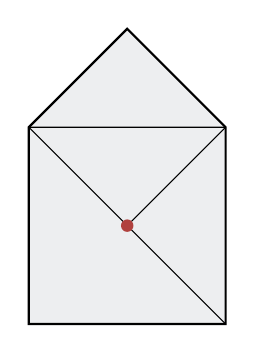
\begin{tikzpicture}[scale=1.25]
\fill[ink!8] (0,0)--(2,0)--(2,2)--(1,3)--(0,2)--cycle;
\draw[thick] (0,0)--(2,0)--(2,2)--(1,3)--(0,2)--cycle;
\draw (2,0)--(0,2) (0,2)--(2,2) (1,1)--(2,2);
\fill[cr] (1,1) circle (1.8pt);
\end{tikzpicture}
\end{column}
\end{columns}
\end{frame}

%======================================================================
\begin{frame}{Monsky's theorem (1970)}
\begin{columns}[c]
\begin{column}{0.5\textwidth}
\begin{block}{Theorem (Monsky)}
A square cannot be dissected into an \textbf{odd} number of triangles of equal area.
\end{block}
\end{column}
\begin{column}{0.46\textwidth}
\centering
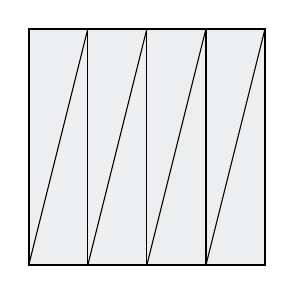
\begin{tikzpicture}[scale=3]
\fill[ink!8] (0,0) rectangle (1,1);
\draw[thick] (0,0) rectangle (1,1);
\foreach \x in {0.25,0.5,0.75} \draw (\x,0)--(\x,1);
\foreach \x in {0,0.25,0.5,0.75} \draw (\x,0)--(\x+0.25,1);
\end{tikzpicture}

\smallskip
{\small A square can be dissected into an arbitrary even number of triangles.}
\end{column}
\end{columns}
\end{frame}

%======================================================================
\begin{frame}{Special polygons}
Orient the boundary of $P$ counter-clockwise. Its sides become \emph{edge vectors}.

\medskip
$P$ is \textbf{special} if, for every line, the edge vectors of $P$ parallel to it sum to $0$.

\vfill
\begin{center}
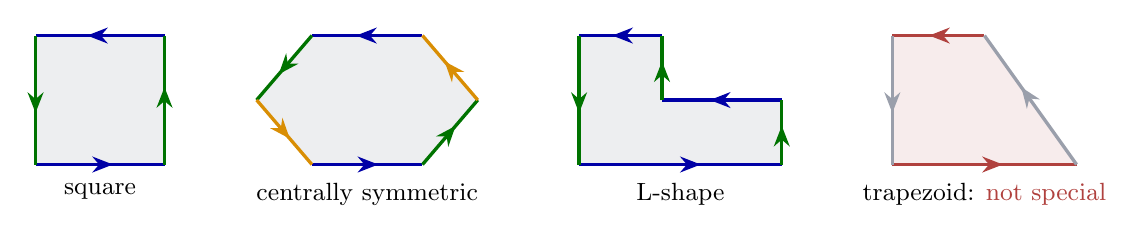
\begin{tikzpicture}[scale=1.17,e/.style={very thick,midarrow}]
\begin{scope}
\fill[ink!8] (0,0) rectangle (1.4,1.4);
\draw[e,cb] (0,0)--(1.4,0); \draw[e,cb] (1.4,1.4)--(0,1.4);
\draw[e,cg] (1.4,0)--(1.4,1.4); \draw[e,cg] (0,1.4)--(0,0);
\node[below] at (0.7,-0.1) {\small square};
\end{scope}
\begin{scope}[xshift=2.4cm]
\fill[ink!8] (0.6,0)--(1.8,0)--(2.4,0.7)--(1.8,1.4)--(0.6,1.4)--(0,0.7)--cycle;
\draw[e,cb] (0.6,0)--(1.8,0); \draw[e,cb] (1.8,1.4)--(0.6,1.4);
\draw[e,cg] (1.8,0)--(2.4,0.7); \draw[e,cg] (0.6,1.4)--(0,0.7);
\draw[e,accent2] (2.4,0.7)--(1.8,1.4); \draw[e,accent2] (0,0.7)--(0.6,0);
\node[below] at (1.2,-0.1) {\small centrally symmetric};
\end{scope}
\begin{scope}[xshift=5.9cm]
\fill[ink!8] (0,0)--(2.2,0)--(2.2,0.7)--(0.9,0.7)--(0.9,1.4)--(0,1.4)--cycle;
\draw[e,cb] (0,0)--(2.2,0); \draw[e,cb] (2.2,0.7)--(0.9,0.7); \draw[e,cb] (0.9,1.4)--(0,1.4);
\draw[e,cg] (2.2,0)--(2.2,0.7); \draw[e,cg] (0.9,0.7)--(0.9,1.4); \draw[e,cg] (0,1.4)--(0,0);
\node[below] at (1.1,-0.1) {\small L-shape};
\end{scope}
\begin{scope}[xshift=9.3cm]
\fill[cr!10] (0,0)--(2,0)--(1,1.4)--(0,1.4)--cycle;
\draw[e,cr] (0,0)--(2,0); \draw[e,cr] (1,1.4)--(0,1.4);
\draw[e,ink!45] (2,0)--(1,1.4); \draw[e,ink!45] (0,1.4)--(0,0);
\node[below] at (1,-0.1) {\small trapezoid: \textcolor{cr}{not special}};
\end{scope}
\end{tikzpicture}
\end{center}
\vfill
\end{frame}

%======================================================================
\begin{frame}{Stein's conjecture}
\vfill
\begin{block}{Conjecture (Stein, 2000)}
A special polygon cannot be dissected into an odd number of triangles of equal area.
\end{block}

\bigskip
\begin{itemize}
\item The square is special, so this generalises Monsky's theorem.
\item We prove it in full generality.
\end{itemize}
\vfill
\end{frame}

%======================================================================
\begin{frame}{Previous results}
\vspace*{3mm}
\centering
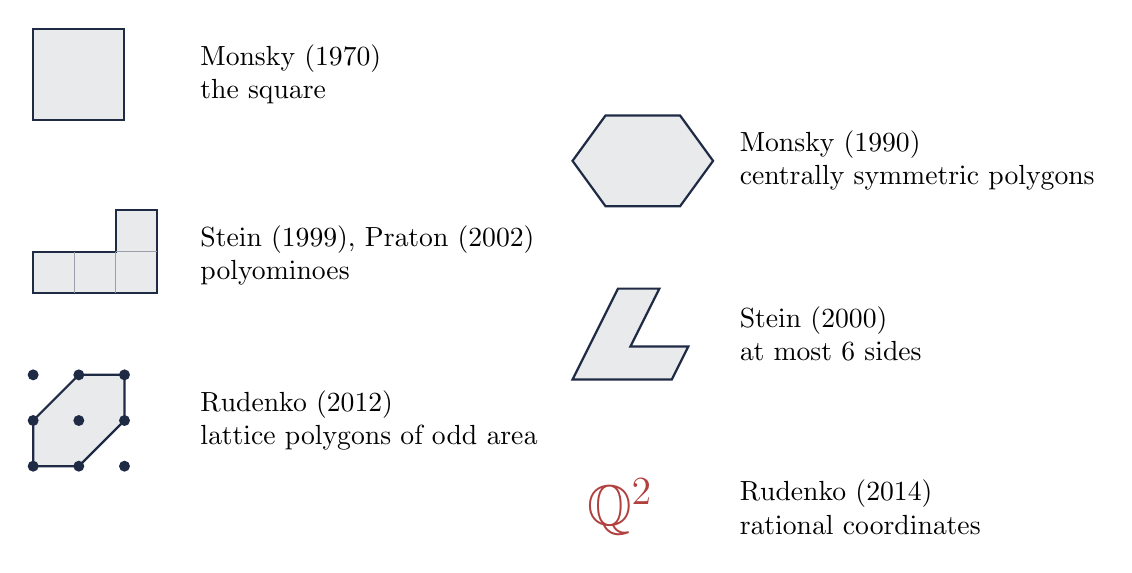
\begin{tikzpicture}[ic/.style={thick,draw=ink,fill=ink!10},lab/.style={anchor=west,align=left},labr/.style={lab}]
% each entry: icon in a 1.1cm box at (x,y), label to its right; entries alternate left/right
\def\S{2.1}
% 1 square
\begin{scope}[shift={(0,0)}]
 \draw[ic,scale=\S] (0,0) rectangle (0.55,0.55);
 \node[lab] at (2.0,0.58) {Monsky (1970)\\ the square};
\end{scope}
% 2 hexagon
\begin{scope}[shift={(6.85,-1.1)}]
 \draw[ic,scale=\S] (0.2,0)--(0.65,0)--(0.85,0.275)--(0.65,0.55)--(0.2,0.55)--(0,0.275)--cycle;
 \node[labr] at (2.0,0.58) {Monsky (1990)\\ centrally symmetric polygons};
\end{scope}
% 3 polyomino
\begin{scope}[shift={(0,-2.2)}]
 \begin{scope}[scale=\S]
 \draw[ic] (0,0)--(0.75,0)--(0.75,0.5)--(0.5,0.5)--(0.5,0.25)--(0,0.25)--cycle;
 \draw[ink!45] (0.25,0)--(0.25,0.25) (0.5,0)--(0.5,0.25) (0.5,0.25)--(0.75,0.25);
 \end{scope}
 \node[lab] at (2.0,0.48) {Stein (1999), Praton (2002)\\ polyominoes};
\end{scope}
% 4 hexagon with at most 6 sides
\begin{scope}[shift={(6.85,-3.3)}]
 \draw[ic,scale=\S] (0,0)--(0.6,0)--(0.7,0.2)--(0.35,0.2)--(0.525,0.55)--(0.275,0.55)--cycle;
 \node[labr] at (2.0,0.58) {Stein (2000)\\ at most $6$ sides};
\end{scope}
% 5 lattice polygon
\begin{scope}[shift={(0,-4.4)}]
 \begin{scope}[scale=0.58]
 \draw[ic] (0,0)--(1,0)--(2,1)--(2,2)--(1,2)--(0,1)--cycle; % lattice hexagon, area 3
 \foreach \x in {0,1,2} \foreach \y in {0,1,2} \fill[ink] (\x,\y) circle[radius=0.12];
 \end{scope}
 \node[lab] at (2.0,0.58) {Rudenko (2012)\\ lattice polygons of odd area};
\end{scope}
% 6 rationals
\begin{scope}[shift={(6.85,-5.5)}]
 \node[accent,font=\huge] at (0.6,0.58) {$\Q^2$};
 \node[labr] at (2.0,0.58) {Rudenko (2014)\\ rational coordinates};
\end{scope}
\end{tikzpicture}
\vspace*{-9mm}
\end{frame}

%======================================================================
\begin{frame}{Why previous results are unsatisfactory}
\vfill
\begin{itemize}
\item \textbf{Heavy machinery:} 3-colourings, Sperner's lemma, homology, flows on graphs.
\bigskip
\item \textbf{No full generality:} each result restricts the shape or the coordinates.
\end{itemize}
\vfill
\end{frame}



%======================================================================
\begin{frame}{The key inequality}
\textbf{Valuation} on a field $K$: \; $v\colon K\to\Gamma\cup\{\infty\}$, \, $\Gamma$ a totally ordered abelian group, with
\[
v(x)=\infty\iff x=0,\qquad v(xy)=v(x)+v(y),\qquad v(x+y)\ge\min\bigl(v(x),v(y)\bigr).
\]

\vfill
\begin{block}{Key Proposition}
For every dissection of a special polygon $P$ into triangles of equal area $a$ and every valuation $v$ on $\R$:
\[
v(2\Area P)\ \ge\ v(2)+v(2a).
\]
\end{block}
\vfill
\end{frame}

%======================================================================
\begin{frame}{Key Proposition $\Rightarrow$ Stein's conjecture}
\vfill
\begin{block}{Key Proposition}
For every dissection of a special polygon $P$ into triangles of equal area $a$ and every valuation $v$ on $\R$:
\[
v(2\Area P)\ \ge\ v(2)+v(2a).
\]
\end{block}
\vfill
Take a dissection of a special polygon $P$ into $n$ triangles of equal area $a$, and a valuation with $v(2)>0$. Then $2\Area P=n\cdot 2a$, so
\[
v(n)+v(2a)\ \ge\ v(2)+v(2a)\quad\Longrightarrow\quad v(n)\ge v(2)>0\quad\Longrightarrow\quad 2\mid n .
\]
\vfill
\end{frame}

%======================================================================
\begin{frame}{Triangles as vector cycles}
\begin{center}
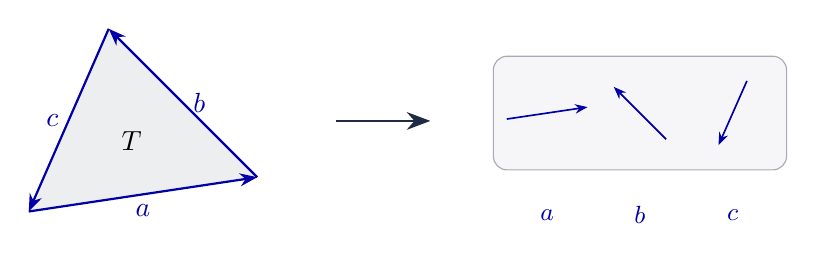
\begin{tikzpicture}
\begin{scope}[scale=1.45]
\coordinate (p) at (0,0); \coordinate (q) at (2,0.3); \coordinate (r) at (0.7,1.6);
\fill[ink!8] (p)--(q)--(r)--cycle;
\draw[vec,cb] (p)--(q) node[midway,below] {$a$};
\draw[vec,cb] (q)--(r) node[midway,right] {$b$};
\draw[vec,cb] (r)--(p) node[midway,left] {$c$};
\node at (0.9,0.62) {$T$};
\end{scope}
\draw[-{Stealth[length=3mm]},thick,ink] (3.9,1.15)--(5.1,1.15);
\begin{scope}[shift={(5.9,1.25)},scale=1.9]
\seq{0}{0}{0.54/0.08/sb, -0.35/0.35/sb, -0.19/-0.43/sb}
\slab[cb]{0}{1}{$a$}\slab[cb]{0}{2}{$b$}\slab[cb]{0}{3}{$c$}
\end{scope}
\end{tikzpicture}
\end{center}

\vspace{-2mm}
\[
\text{\emph{vector cycle}: a sequence } c=(c_1,\dots,c_r) \text{ with } \sum_i c_i=0,\qquad\quad \ar c=\sum_{i<j}\det(c_i,c_j)
\]
\begin{center}
Counter-clockwise triangle: \quad $\ar{(a,b,c)}=2\Area T$
\end{center}
\end{frame}

%======================================================================
\begin{frame}{A dissection becomes a family of cycles}
\begin{columns}[c]
\begin{column}{0.3\textwidth}
\centering
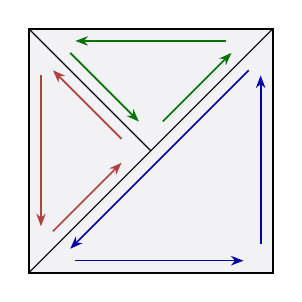
\begin{tikzpicture}[scale=3.1]
\fill[ink!6] (0,0) rectangle (1,1);
\draw[thick] (0,0) rectangle (1,1);
\draw (0,0)--(1,1) (0,1)--(0.5,0.5);
% (0,0),(1,0),(1,1)
\draw[sb] (0.191,0.050)--(0.880,0.050); \draw[sb] (0.950,0.120)--(0.950,0.809); \draw[sb] (0.901,0.830)--(0.170,0.099);
% (0,0),(0.5,0.5),(0,1)
\draw[sr] (0.099,0.170)--(0.380,0.451); \draw[sr] (0.380,0.549)--(0.099,0.830); \draw[sr] (0.050,0.809)--(0.050,0.191);
% (0.5,0.5),(1,1),(0,1)
\draw[sg] (0.549,0.620)--(0.830,0.901); \draw[sg] (0.809,0.950)--(0.191,0.950); \draw[sg] (0.170,0.901)--(0.451,0.620);
\end{tikzpicture}
\end{column}
\begin{column}{0.68\textwidth}
\centering
A \textbf{family} of vector cycles

\smallskip
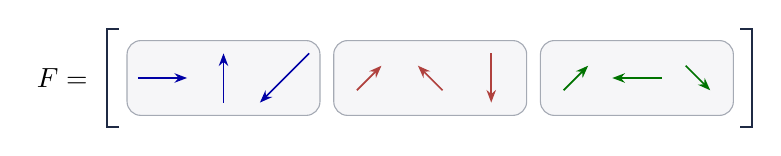
\begin{tikzpicture}[scale=1.25]
\node[left] at (-0.3,0) {$F=$};
\Fam{-0.2}{6.35}{0}
\seq{0}{0}{0.5/0/sb, 0/0.5/sb, -0.5/-0.5/sb}
\seq{2.1}{0}{0.25/0.25/sr, -0.25/0.25/sr, 0/-0.5/sr}
\seq{4.2}{0}{0.25/0.25/sg, -0.5/0/sg, 0.25/-0.25/sg}
\end{tikzpicture}

\smallskip
$S(F)=\sum_{c\in F}\ar c=2\Area P$

\medskip
\textbf{Balanced}: for every line, the vectors parallel to it sum to $0$.

\smallskip
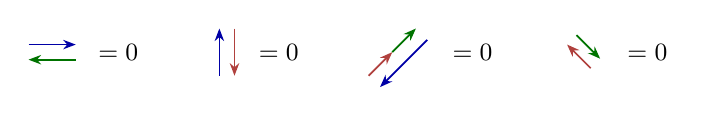
\begin{tikzpicture}[scale=1.2]
\draw[sb] (0,0.08)--(0.5,0.08); \draw[sg] (0.5,-0.08)--(0,-0.08);
\node[font=\small] at (0.95,0) {$=0$};
\begin{scope}[xshift=2.1cm]
\draw[sb] (-0.08,-0.25)--(-0.08,0.25); \draw[sr] (0.08,0.25)--(0.08,-0.25);
\node[font=\small] at (0.55,0) {$=0$};
\end{scope}
\begin{scope}[xshift=3.6cm]
\draw[sr] (0,-0.25)--(0.25,0); \draw[sg] (0.25,0)--(0.5,0.25); \draw[sb] (0.62,0.13)--(0.12,-0.37);
\node[font=\small] at (1.1,0) {$=0$};
\end{scope}
\begin{scope}[xshift=5.7cm]
\draw[sr] (0.25,-0.17)--(0,0.08); \draw[sg] (0.1,0.18)--(0.35,-0.07);
\node[font=\small] at (0.85,0) {$=0$};
\end{scope}
\end{tikzpicture}
\end{column}
\end{columns}
\end{frame}

%======================================================================
\begin{frame}{Three moves}
\centering
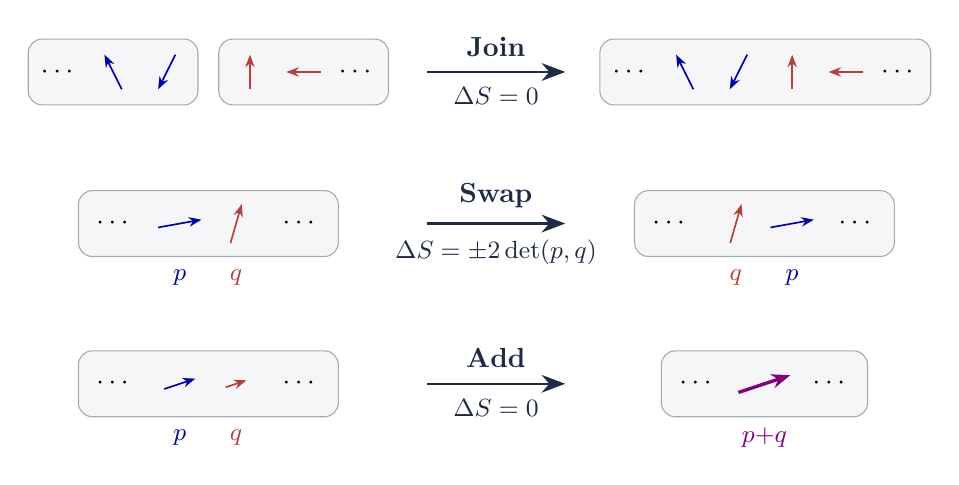
\begin{tikzpicture}[scale=1.1]
% Join
\seq{0}{0}{0.4/0/hid, -0.2/0.4/sb, -0.2/-0.4/sb}
\seq{2.2}{0}{0/0.4/sr, -0.4/0/sr, 0.4/-0.4/hid}
\node at (0.36,0) {$\cdots$}; \node at (3.8,0) {$\cdots$};
\mv{0}{Join}{$\Delta S=0$}
\seq{6.6}{0}{0.4/0/hid, -0.2/0.4/sb, -0.2/-0.4/sb, 0/0.4/sr, -0.4/0/sr, 0.4/-0.4/hid}
\node at (6.96,0) {$\cdots$}; \node at (10.06,0) {$\cdots$};
% Swap
\begin{scope}[yshift=-1.75cm]
\seqframe{0.58}{0}{3}
\node at (1.0,0) {$\cdots$}; \cv[sb]{1.75}{0}{0.5}{0.09} \cv[sr]{2.4}{0}{0.13}{0.45} \node at (3.15,0) {$\cdots$};
\node[cb,font=\small] at (1.75,-0.62) {$p$}; \node[cr,font=\small] at (2.4,-0.62) {$q$};
\mv{0}{Swap}{$\Delta S=\pm2\det(p,q)$}
\seqframe{7.0}{0}{3}
\node at (7.42,0) {$\cdots$}; \cv[sr]{8.17}{0}{0.13}{0.45} \cv[sb]{8.82}{0}{0.5}{0.09} \node at (9.57,0) {$\cdots$};
\node[cr,font=\small] at (8.17,-0.62) {$q$}; \node[cb,font=\small] at (8.82,-0.62) {$p$};
\end{scope}
% Add
\begin{scope}[yshift=-3.6cm]
\seqframe{0.58}{0}{3}
\node at (1.0,0) {$\cdots$}; \cv[sb]{1.75}{0}{0.36}{0.12} \cv[sr]{2.4}{0}{0.24}{0.08} \node at (3.15,0) {$\cdots$};
\node[cb,font=\small] at (1.75,-0.62) {$p$}; \node[cr,font=\small] at (2.4,-0.62) {$q$};
\mv{0}{Add}{$\Delta S=0$}
\seqframe{7.31}{0}{2.38}
\node at (7.73,0) {$\cdots$}; \cv[sumv]{8.5}{0}{0.6}{0.2} \node at (9.27,0) {$\cdots$};
\node[violet,font=\small] at (8.5,-0.62) {$p{+}q$};
\end{scope}
\end{tikzpicture}
\end{frame}

%======================================================================
\begin{frame}{The induction: setup}
\vfill
\[
I=\{x\in\R\mid v(x)\ge v(2)+v(2a)\}\quad\text{\small(an additive subgroup)}
\]

\vfill
\begin{center}
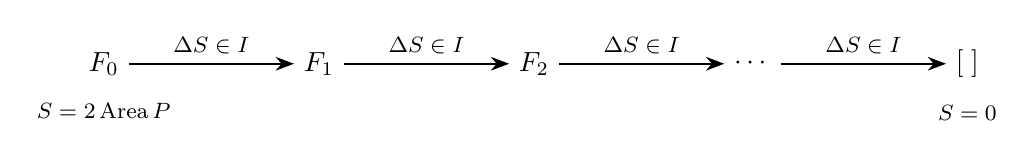
\begin{tikzpicture}[node distance=2.1cm]
\node (a) {$F_0$};
\node[right=of a] (b) {$F_1$};
\node[right=of b] (c) {$F_2$};
\node[right=of c] (d) {$\cdots$};
\node[right=of d] (e) {$[\;]$};
\foreach \x/\y in {a/b,b/c,c/d,d/e} \draw[-{Stealth},thick] (\x) -- node[above] {\footnotesize $\Delta S\in I$} (\y);
\node[below=3pt of a] {\footnotesize $S=2\Area P$};
\node[below=3pt of e] {\footnotesize $S=0$};
\end{tikzpicture}
\end{center}

\vfill
\begin{center}
\textbf{Goal:} \; show that $2\Area P=S(F_0)$ lies in $I$.
\end{center}
\vfill
\end{frame}

%======================================================================
\begin{frame}{Step 1: the vector of smallest valuation and its partner}
\begin{columns}[c]
\begin{column}{0.47\textwidth}
Take the vector \textcolor{cr}{$u$} with the smallest valuation.

\medskip
It has a partner vector \textcolor{accent2}{$u'$} which is parallel and has the same valuation.

\medskip
We will add those vectors together.
\end{column}
\begin{column}{0.5\textwidth}
\centering
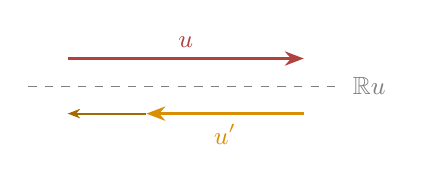
\begin{tikzpicture}[scale=1.25]
\draw[gray,dashed] (-0.4,0)--(2.8,0) node[right] {\small $\R u$};
\draw[longu] (0,0.28)--(2.4,0.28) node[midway,above] {\small $u$};
\draw[longup] (2.4,-0.28)--(0.8,-0.28) node[midway,below] {\small $u'$};
\draw[par,thick] (0.8,-0.28)--(0,-0.28);
\end{tikzpicture}
\end{column}
\end{columns}
\end{frame}


%======================================================================
\begin{frame}{Steps 2--4: join, swap, add}
\vfill
\begin{center}
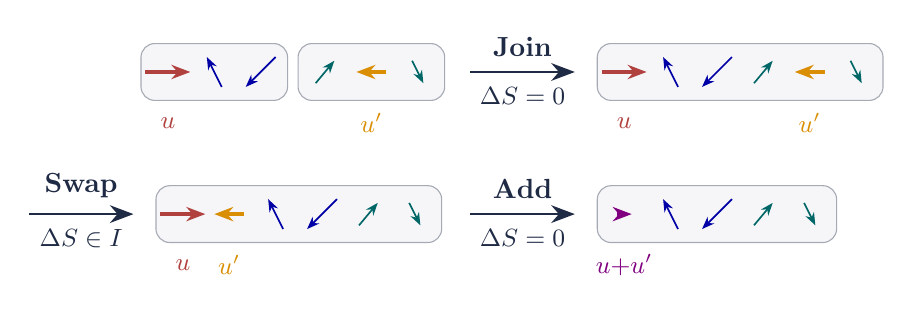
\begin{tikzpicture}[scale=0.95]
\seq{0}{0}{0.6/0/longu, -0.2/0.4/sb, -0.4/-0.4/sb}
\seq{2.1}{0}{0.25/0.3/st, -0.4/0/longup, 0.15/-0.3/st}
\slab[cr]{0}{1}{$u$}\slab[accent2]{2.1}{2}{$u'$}
\draw[next] (4.4,0)--(5.8,0) node[midway,above=2pt] {\textbf{Join}} node[midway,below=2pt,font=\small] {$\Delta S=0$};
\seq{6.1}{0}{0.6/0/longu, -0.2/0.4/sb, -0.4/-0.4/sb, 0.25/0.3/st, -0.4/0/longup, 0.15/-0.3/st}
\slab[cr]{6.1}{1}{$u$}\slab[accent2]{6.1}{5}{$u'$}
\begin{scope}[yshift=-1.9cm]
\draw[next] (-1.5,0)--(-0.1,0) node[midway,above=2pt] {\textbf{Swap}} node[midway,below=2pt,font=\small] {$\Delta S\in I$};
\seq{0.2}{0}{0.6/0/longu, -0.4/0/longup, -0.2/0.4/sb, -0.4/-0.4/sb, 0.25/0.3/st, 0.15/-0.3/st}
\slab[cr]{0.2}{1}{$u$}\slab[accent2]{0.2}{2}{$u'$}
\draw[next] (4.4,0)--(5.8,0) node[midway,above=2pt] {\textbf{Add}} node[midway,below=2pt,font=\small] {$\Delta S=0$};
\seq{6.1}{0}{0.2/0/sumv, -0.2/0.4/sb, -0.4/-0.4/sb, 0.25/0.3/st, 0.15/-0.3/st}
\node[violet,font=\small] at (6.46,-0.68) {$u{+}u'$};
\end{scope}
\end{tikzpicture}
\end{center}

\vfill
\centering
Hence\quad $\boldsymbol{2\Area P=S(F_0)\in I}$.
\vfill
\end{frame}


%======================================================================
\begin{frame}{Main takeaway}
\vfill
\begin{center}
\large A short, elementary proof of Stein's conjecture in full generality.
\end{center}

\bigskip
\begin{itemize}
\item \textbf{Full generality.} Every special polygon, with arbitrary real coordinates. Previous results restricted the shape or the coordinates.
\medskip
\item \textbf{No heavy machinery.} One valuation and determinants. No colourings, Sperner's lemma, homology or flows on graphs.
\end{itemize}
\vfill
\end{frame}


%======================================================================
\begin{frame}{Formalisation in Lean 4}
\vfill
\begin{itemize}
\item The formalised theorem is \textbf{Stein's conjecture}, proved in Lean 4 with Mathlib.
\bigskip
\item The \textbf{official Mathathon statement} of Monsky's theorem follows as a corollary.
\bigskip
\item We checked the formal statement and its definitions ourselves.
\end{itemize}
\vfill
\end{frame}


\end{document}
